\section{Experimental results and discussions}
\label{sec:experimental_results}

Equations \eqref{eq:D_temp_sigma} form the basis of our proposed EM model under time-varying temperature stress. A number of simulations were studied using the approach described above, both in Matlab and COMSOL, considering the varying impact of temperature over time.
In the simulations to be described below, the following input values were used: $Z^*=10$, $\rho=3\times10^{-8} \Omega/m$, $\Omega=8.78\times10^{-30}m^3$, $B=5.5\times10^{10} Pa$, $D_0=5.5\times10^{-5} m^2/s$, $E_a=1.1eV$, $e=1.6\times10^{-19}C$, $k=1.38\times10^{-23}J/K$. The metal wire structure used in our experiment is shown in Fig.~\ref{fig:InterconnectTree}. We assume that the nucleation time is $4\times10^7$ s. And the length of each branch is set to $20\mu m$.

We first apply the COMSOL to compute an accurate numerical solution of \eqref{eq:basic_em}. We set the width of 3D interconnect tree as $10^{-8}m$, considering the thin and narrow interconnect line. Then we use the proposed approach to estimate the stress in MATLAB. Comparisons are shown in Fig.~\ref{fig:SResults}, Fig.~\ref{fig:TResults}, and Fig.~\ref{fig:CResults}.
\subsection{Straight line interconnect tree results}
We first analyze the 3-terminal interconnect tree with two segments with the current flow directions as showed in Fig.\ref{fig:singleline}. Fig.\ref{fig:SResults} shows obtained evolution of the stress distribution. From Fig.\ref{fig:ST1Compare} and Fig.\ref{fig:ST2Compare}, analytical solution obtained with the proposed method fits well to the results of the numerical simulation at every time instance. For a fixed position shown in Fig.\ref{fig:ST1Length} and Fig.\ref{fig:ST2Length}, the stress changes in agreement with the varying temperatures. In the case of square ware temperature, when temperature rises up to $380K$, the stress is going through dramatic changes. On the contrary, when temperature is $320K$, the stress is smoothly continuous. In the case of sine wave temperature, when temperature falls down to below $250K$, the stress has a process of slow change. And average temperature is useless for the interconnect tree analysis. Thermal effects depended on the varying temperature are remarkable.
\begin{figure}[!h]
\centering
\subfigure[]{
\includegraphics[width=0.45\columnwidth]{SStressMatComCompareT1.eps}
\label{fig:ST1Compare}}
\subfigure[]{
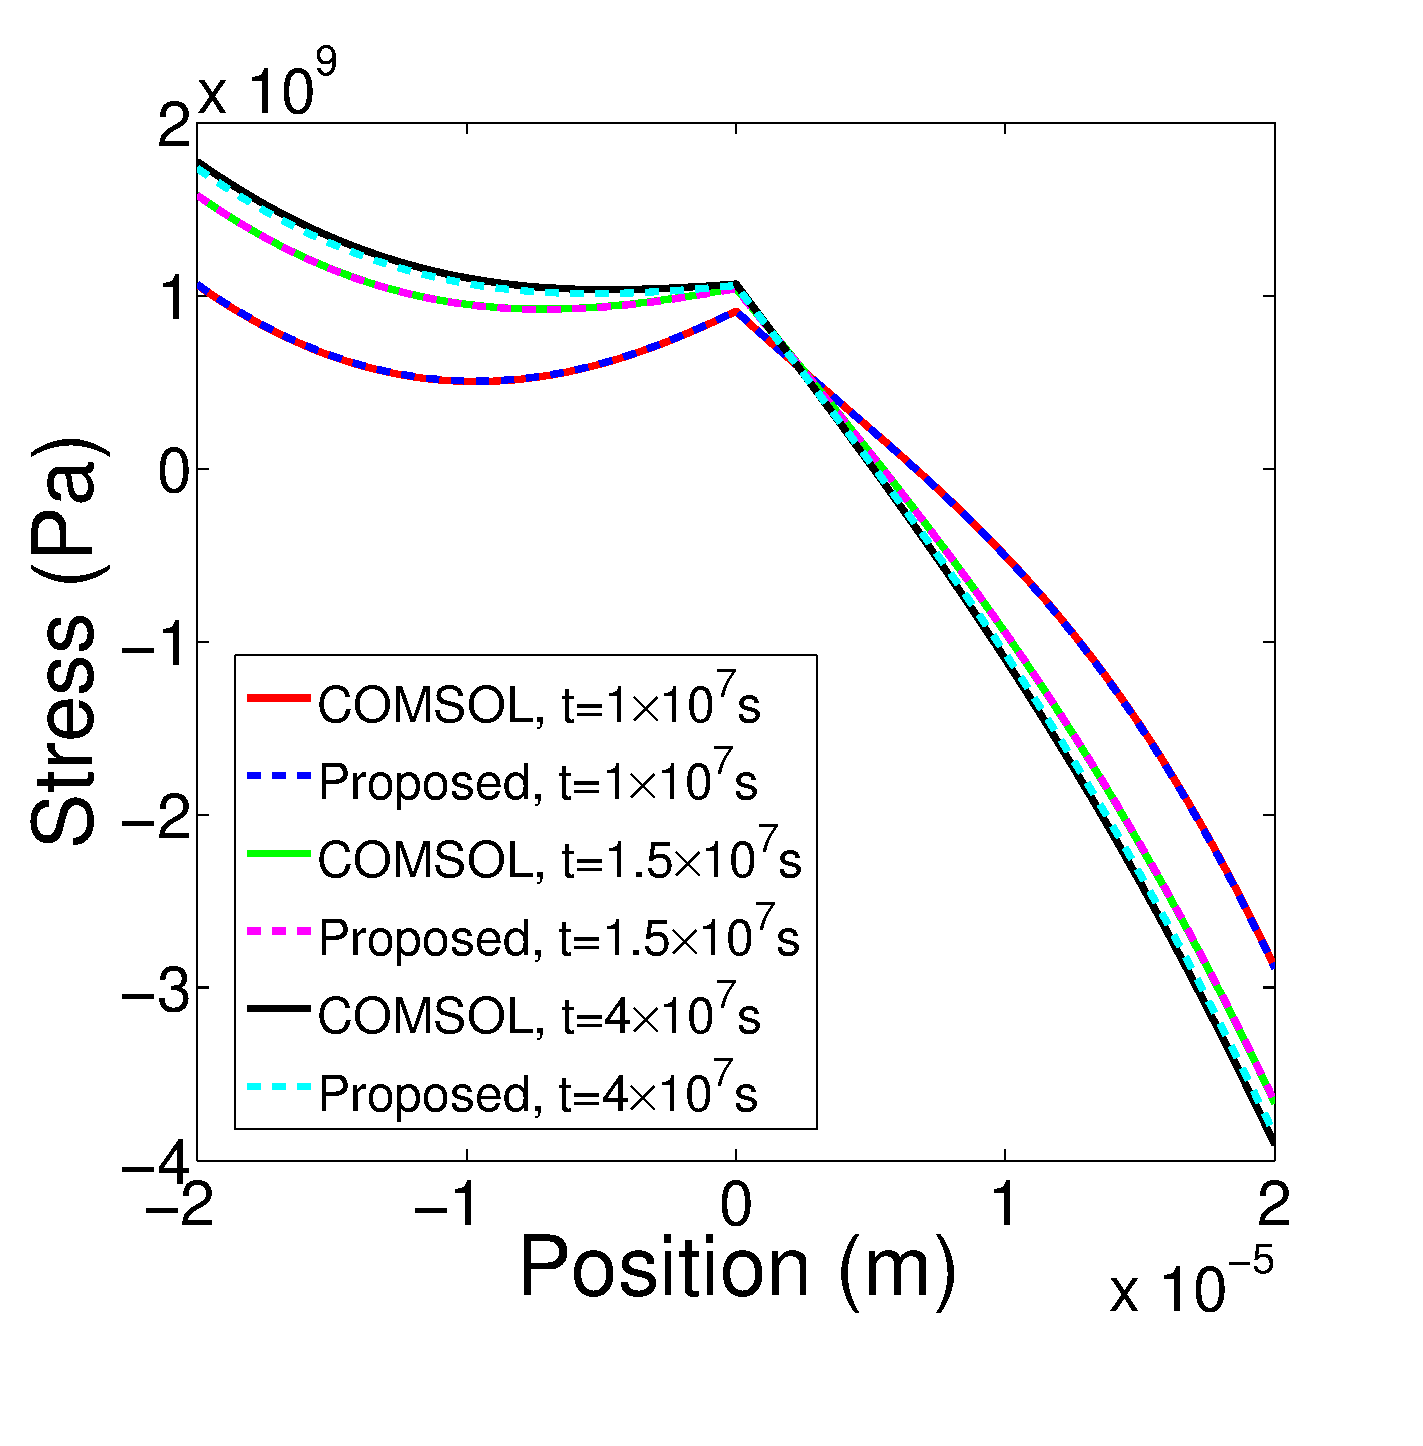
\includegraphics[width=0.45\columnwidth]{SStressMatComCompareT2.eps}
\label{fig:ST2Compare}}
\subfigure[]{
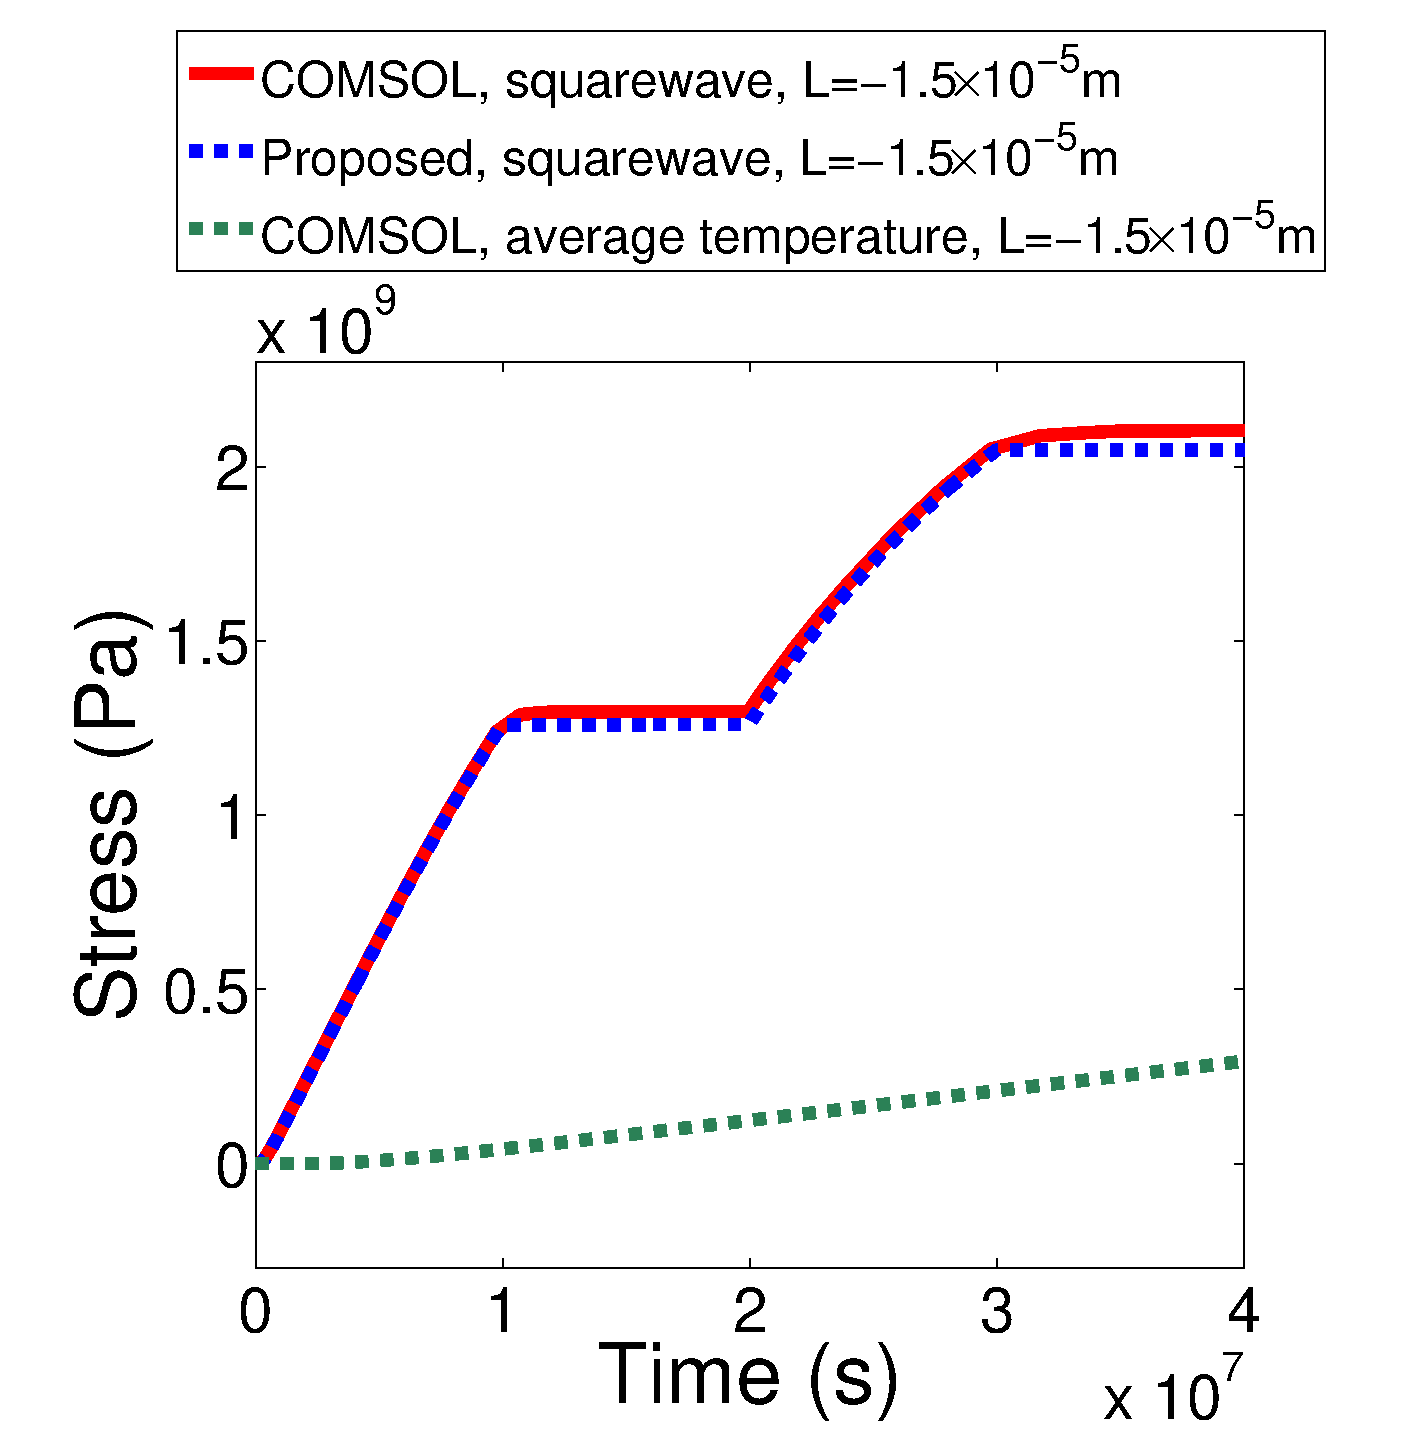
\includegraphics[width=0.45\columnwidth]{SLengthCompareT1.eps}
\label{fig:ST1Length}}
\subfigure[]{
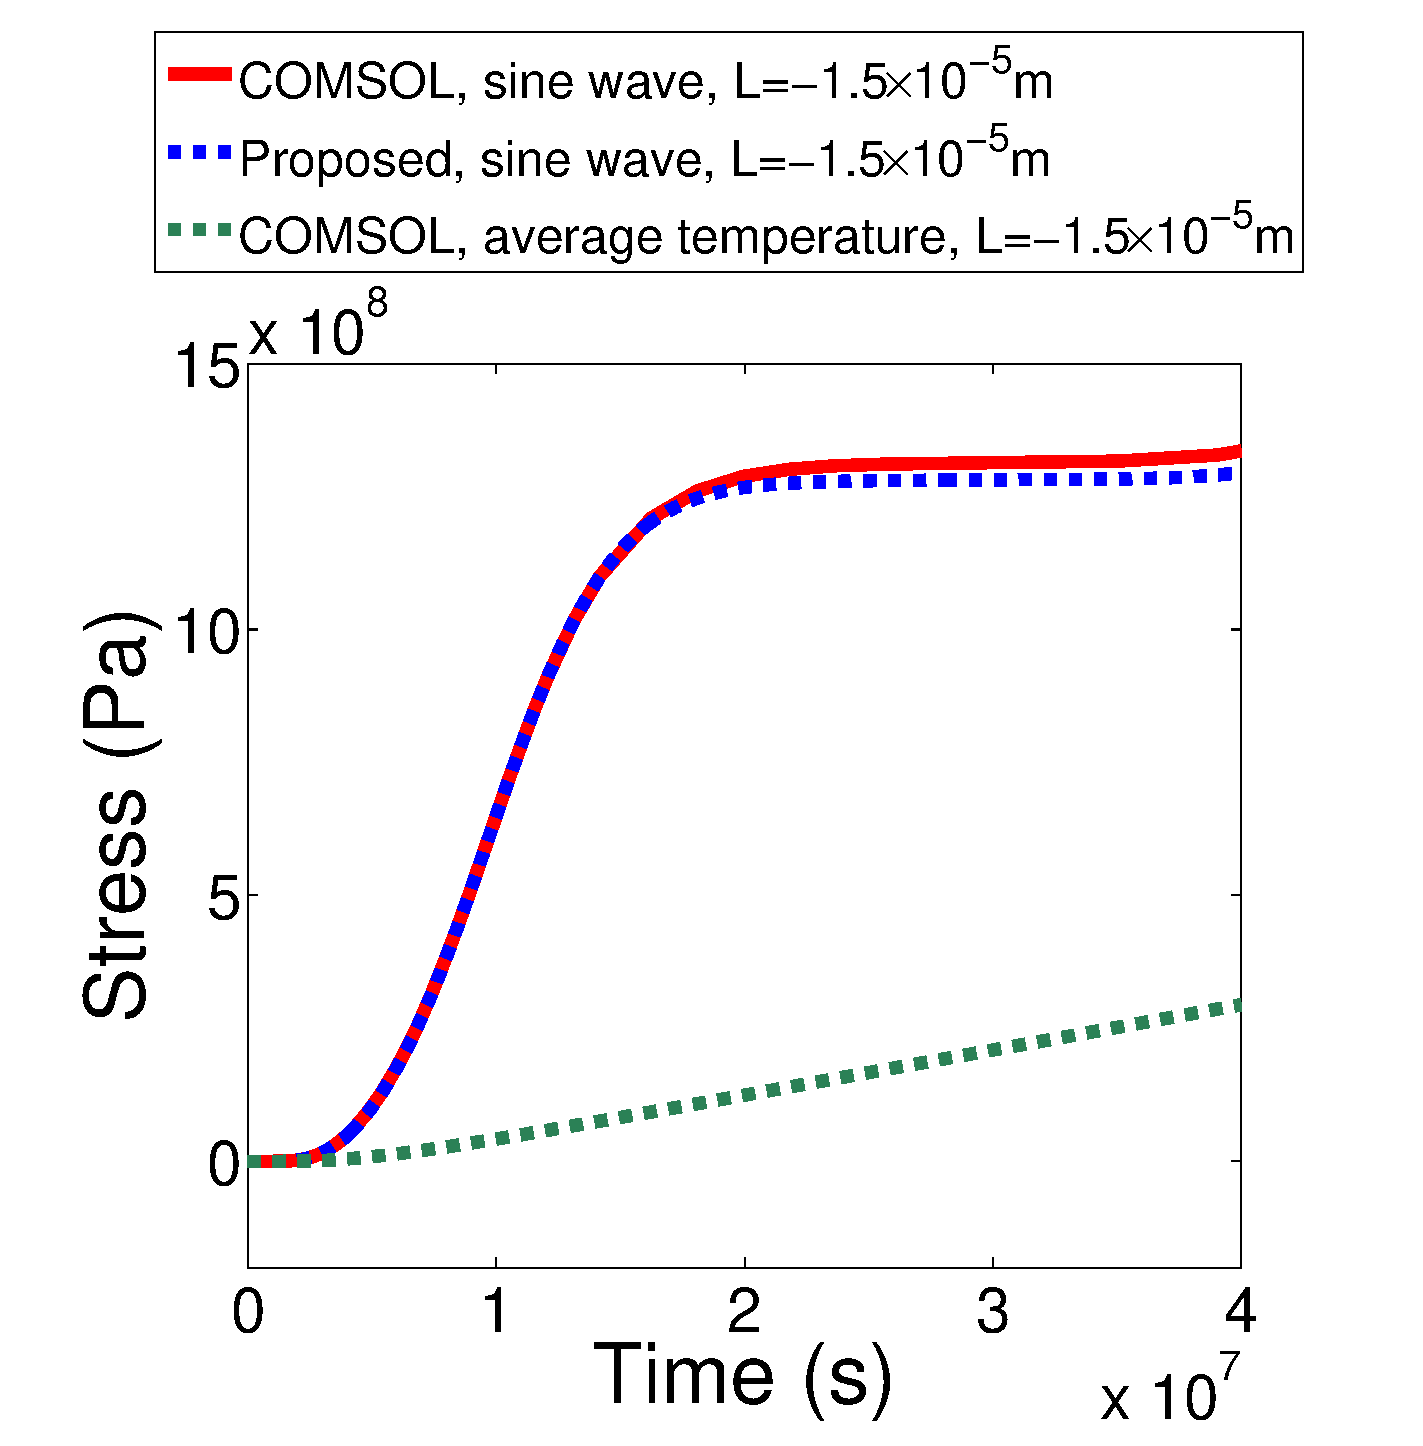
\includegraphics[width=0.45\columnwidth]{SLengthCompareT2.eps}
\label{fig:ST2Length}}
\caption{The experiments results of straight line at changing temperatures, $j_1=2\times10^{10}A/m^2,\;j_2=6\times10^{10}A/m^2$ (a) the comparison of stress evolution at square wave temperature at a fixed time; (b) the comparison of stress evolution at sine wave temperature at a fixed time; (c) the comparison of stress evolution at square wave temperature at a fixed position; (d) the comparison of stress evolution at sine wave temperature at a fixed position}
\label{fig:SResults}
\end{figure}


\subsection{T-shaped interconnect tree results}
As expected in Fig.\ref{fig:TResults}, the stress distribution in the T-shaped tree shown in Fig.\ref{fig:Tshaped}, based on proposed analytical solution, has synchronized movement with numerical simulation in COMSOL. From Fig.\ref{fig:TT1Length} and Fig.\ref{fig:TT2Length},when the T-shaped tree works over $1\times10^{7}s$ in branch $1$, the stress as mild changes. So we just take two time values in Fig.\ref{fig:TT1Compare} and Fig.\ref{fig:TT2Compare}.
\begin{figure}[!h]
\centering
\subfigure[]{
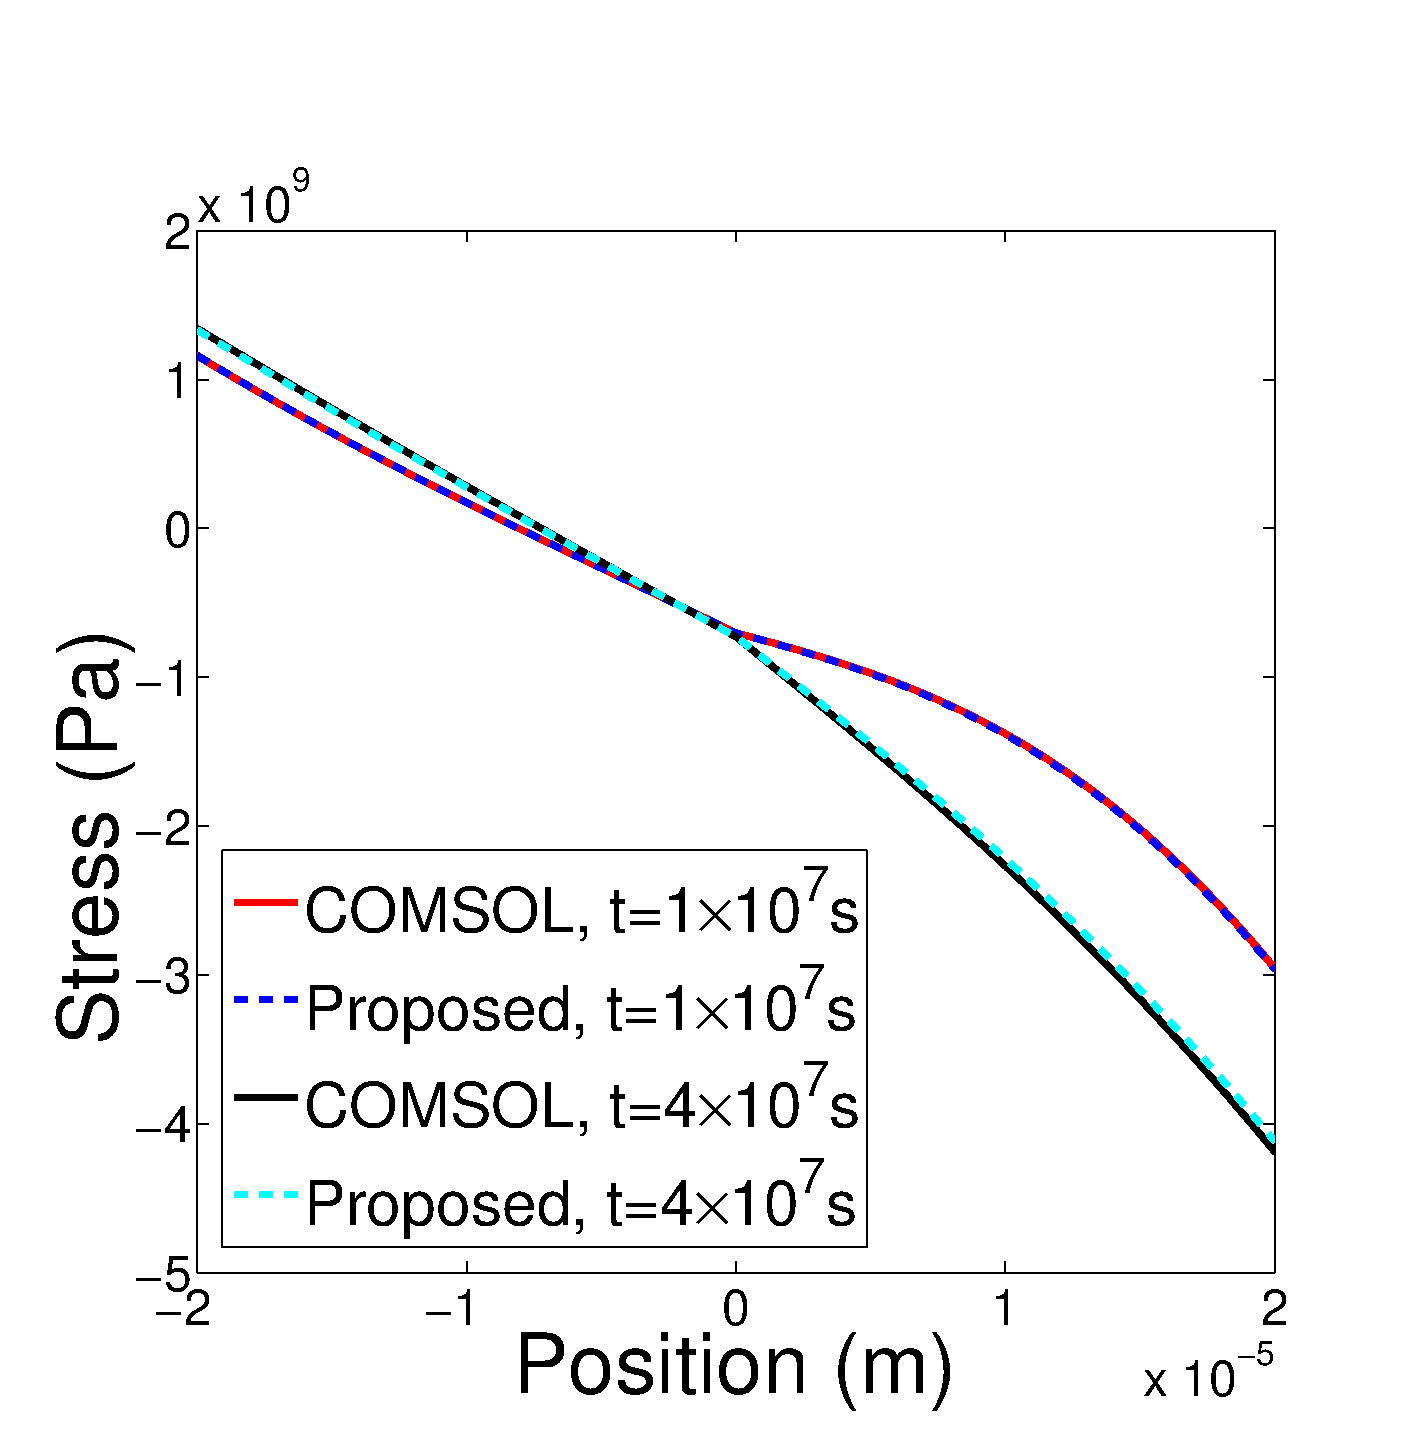
\includegraphics[width=0.45\columnwidth]{TStressMatComCompareT1.eps}
\label{fig:TT1Compare}}
\subfigure[]{
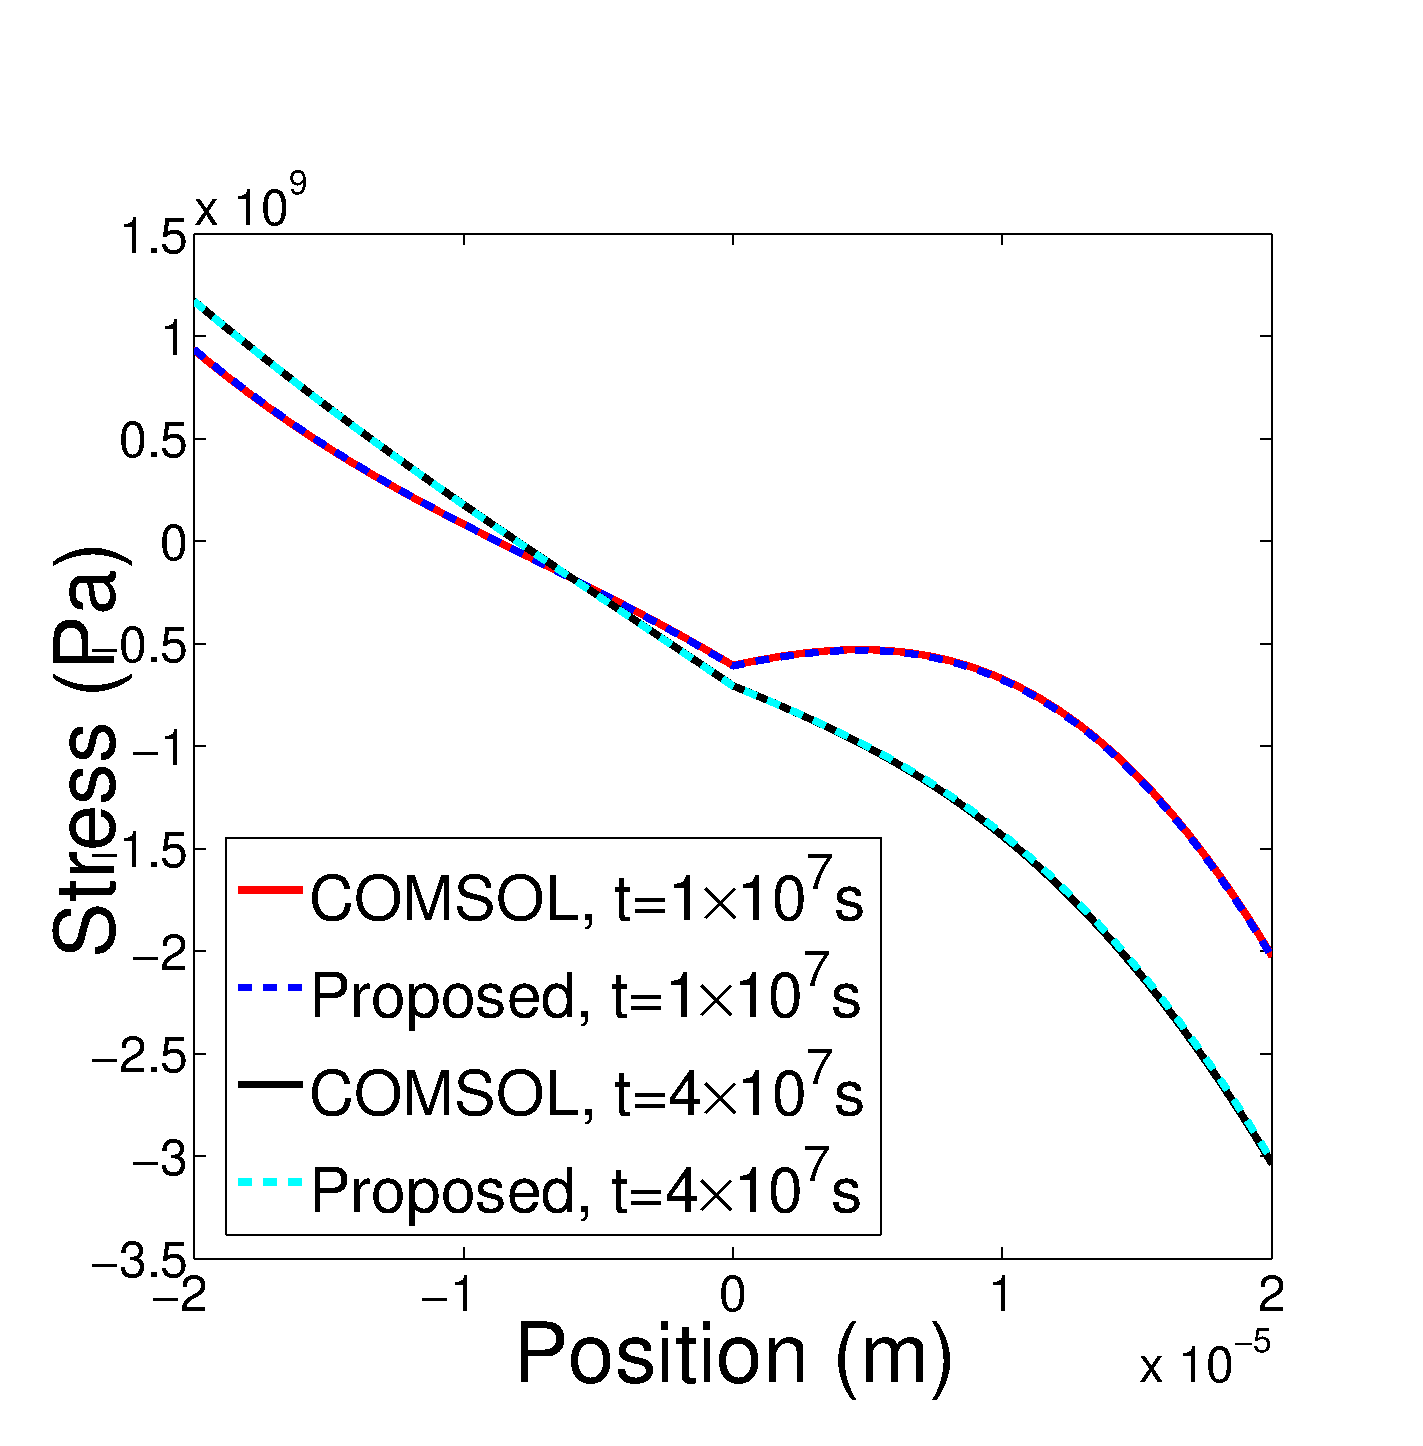
\includegraphics[width=0.45\columnwidth]{TStressMatComCompareT2.eps}
\label{fig:TT2Compare}}
\subfigure[]{
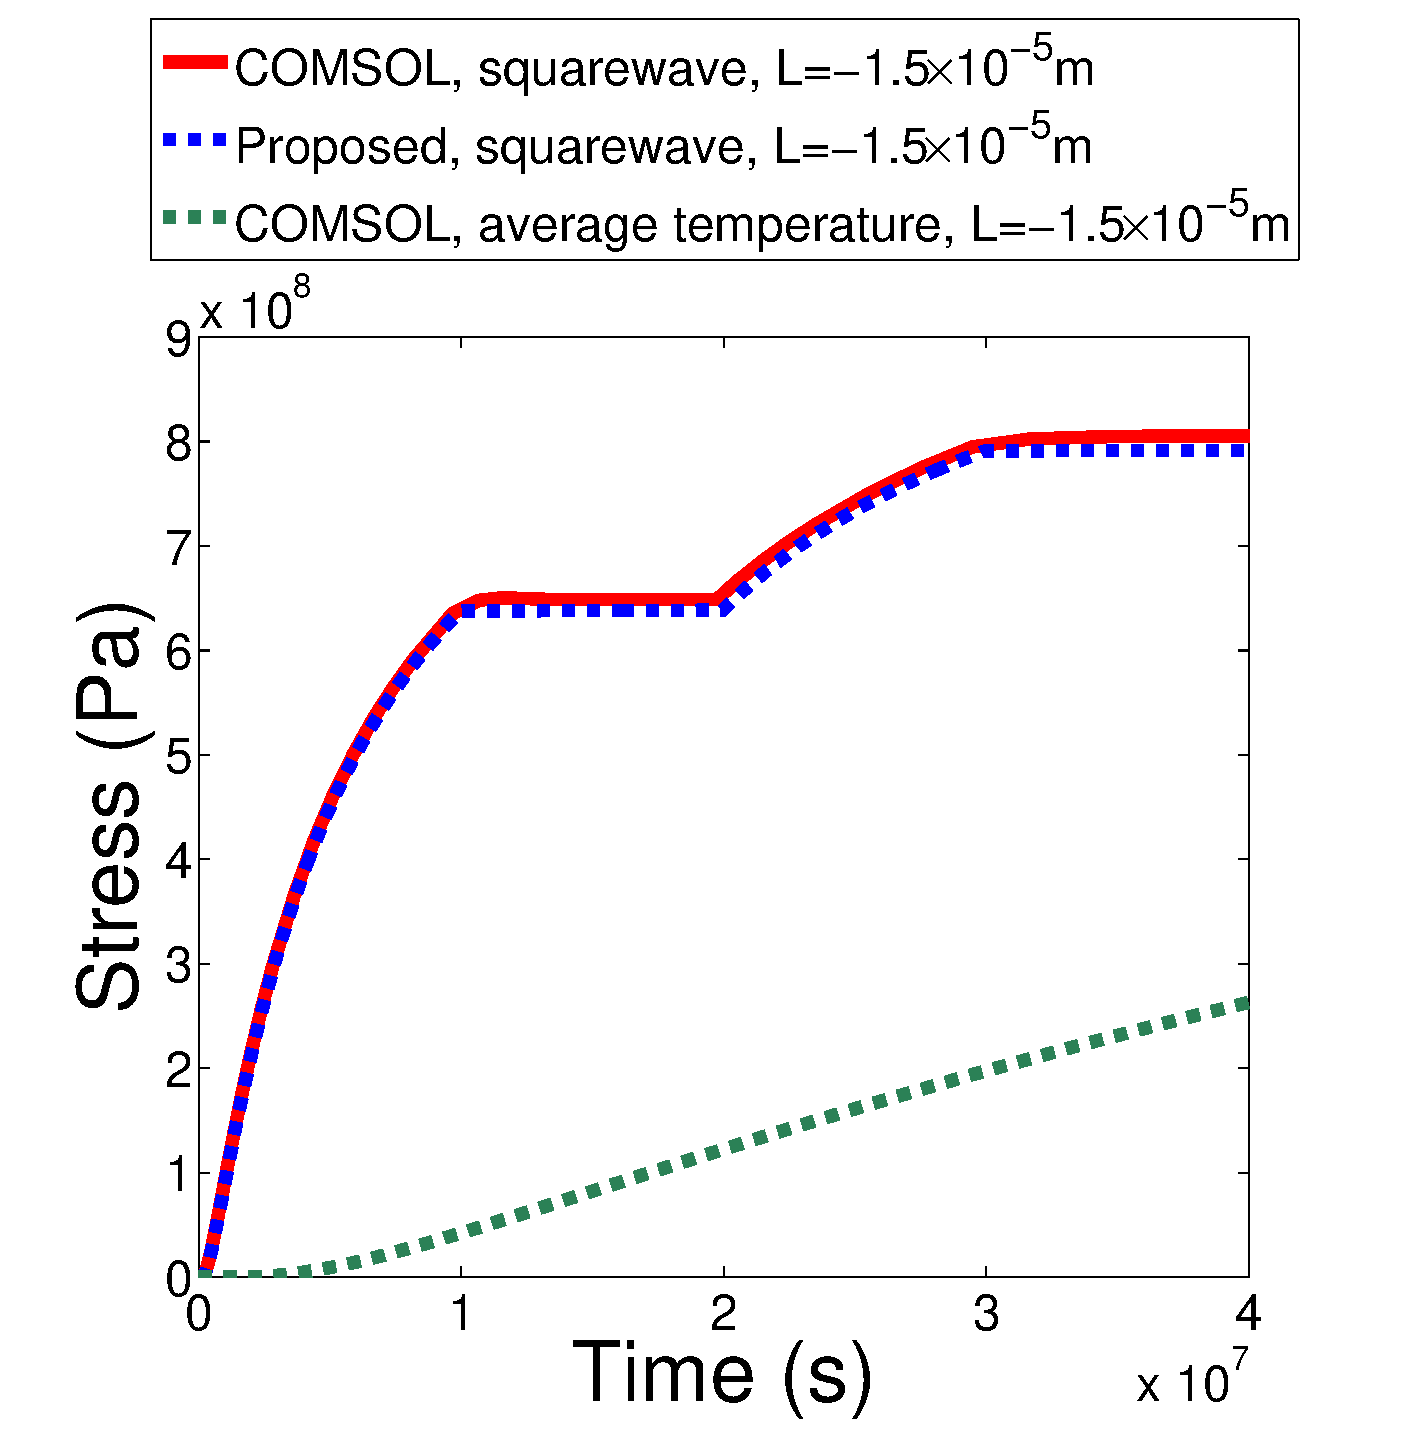
\includegraphics[width=0.45\columnwidth]{TLengthCompareT1.eps}
\label{fig:TT1Length}}
\subfigure[]{
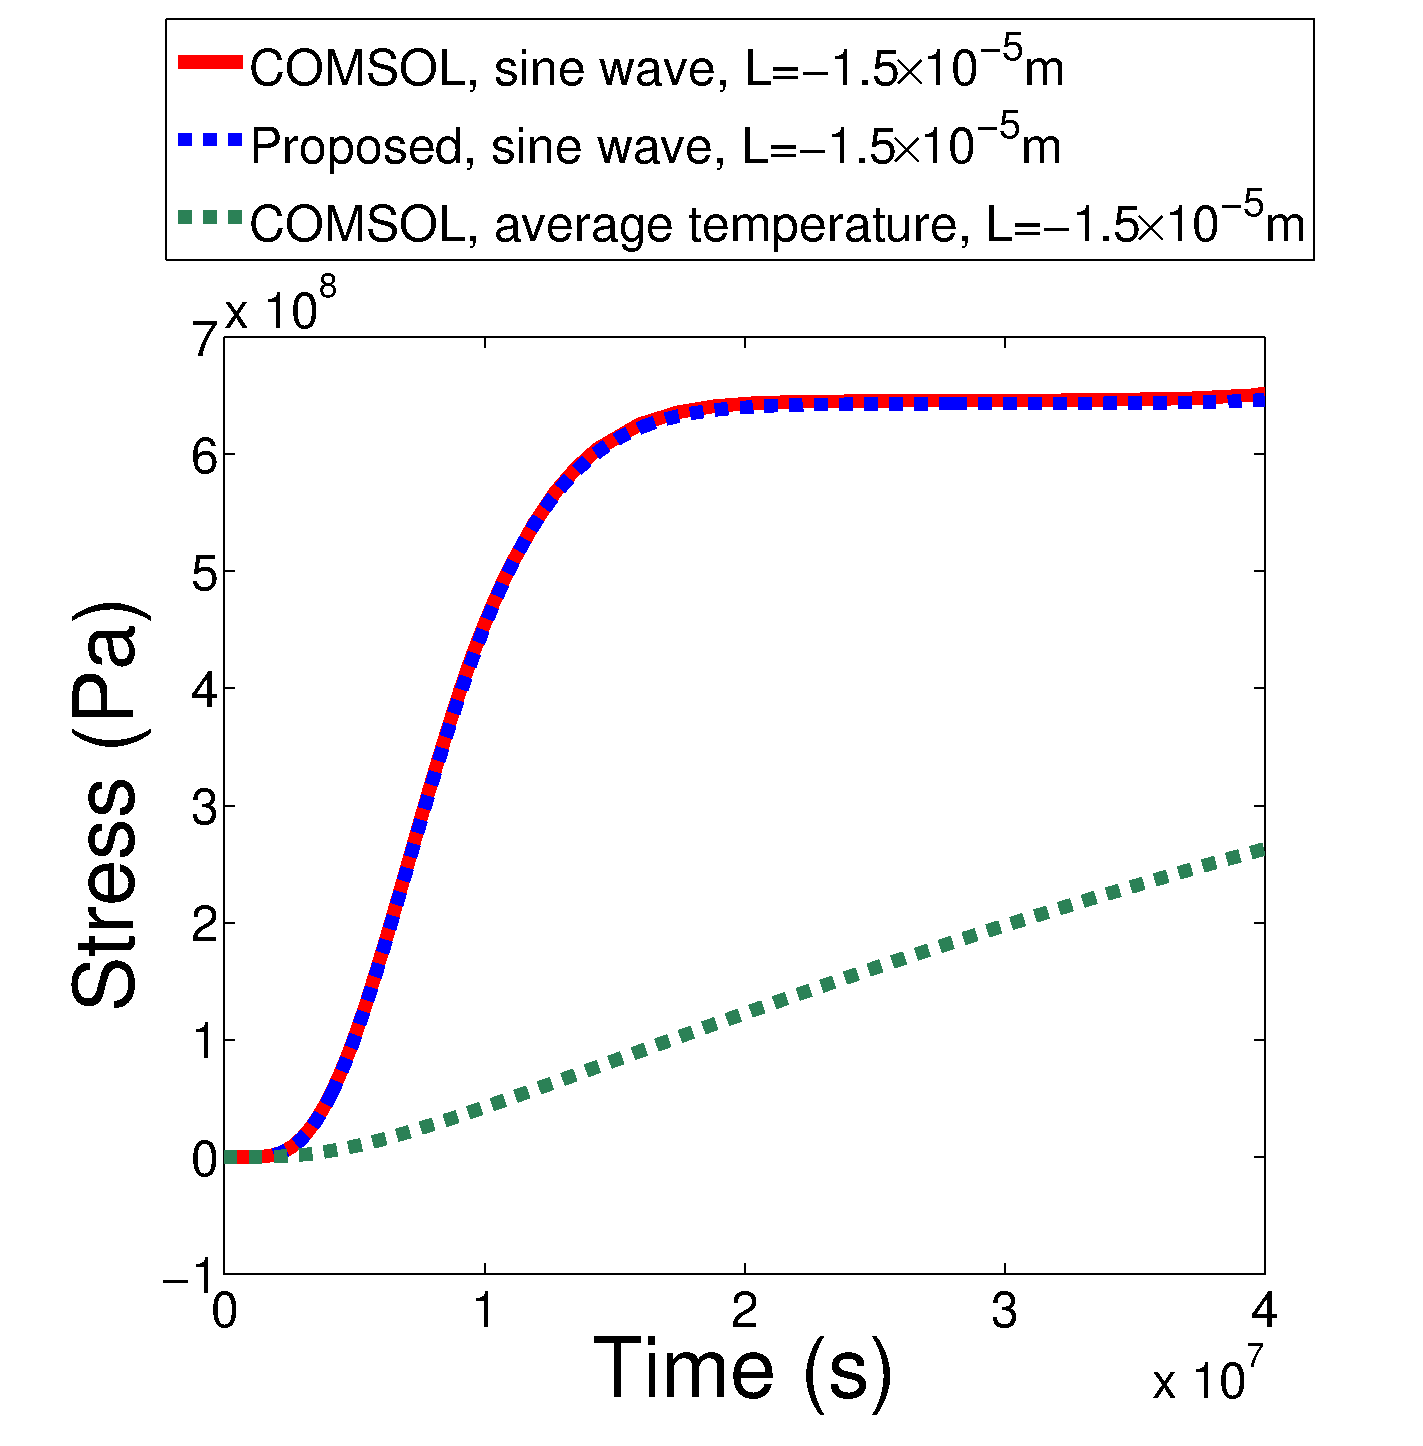
\includegraphics[width=0.45\columnwidth]{TLengthCompareT2.eps}
\label{fig:TT2Length}}
\caption{The experiments results of T-shaped interconnect tree at changing temperatures, $j_1=2\times10^{10}A/m^2,\;j_2=4\times10^{10}A/m^2,\;j_3=6\times10^{10}A/m^2$ (a) the comparison of stress evolution at square wave temperature at a fixed time; (b) the comparison of stress evolution at sine wave temperature at a fixed time; (c) the comparison of stress evolution at square wave temperature at a fixed position; (d) the comparison of stress evolution at sine wave temperature at a fixed position}
\label{fig:TResults}
\end{figure}

\subsection{Cross-shaped interconnect tree results}
From Fig.\ref{fig:CResults} considering the basic tree shown in Fig.\ref{fig:Cshaped}, we can see that the stress evolution of proposed model fits well to those obtained from COMSOL. Without the proposed model, we maybe use the average temperature to estimate the stress evolution.
\begin{figure}[!h]
\centering
\subfigure[]{
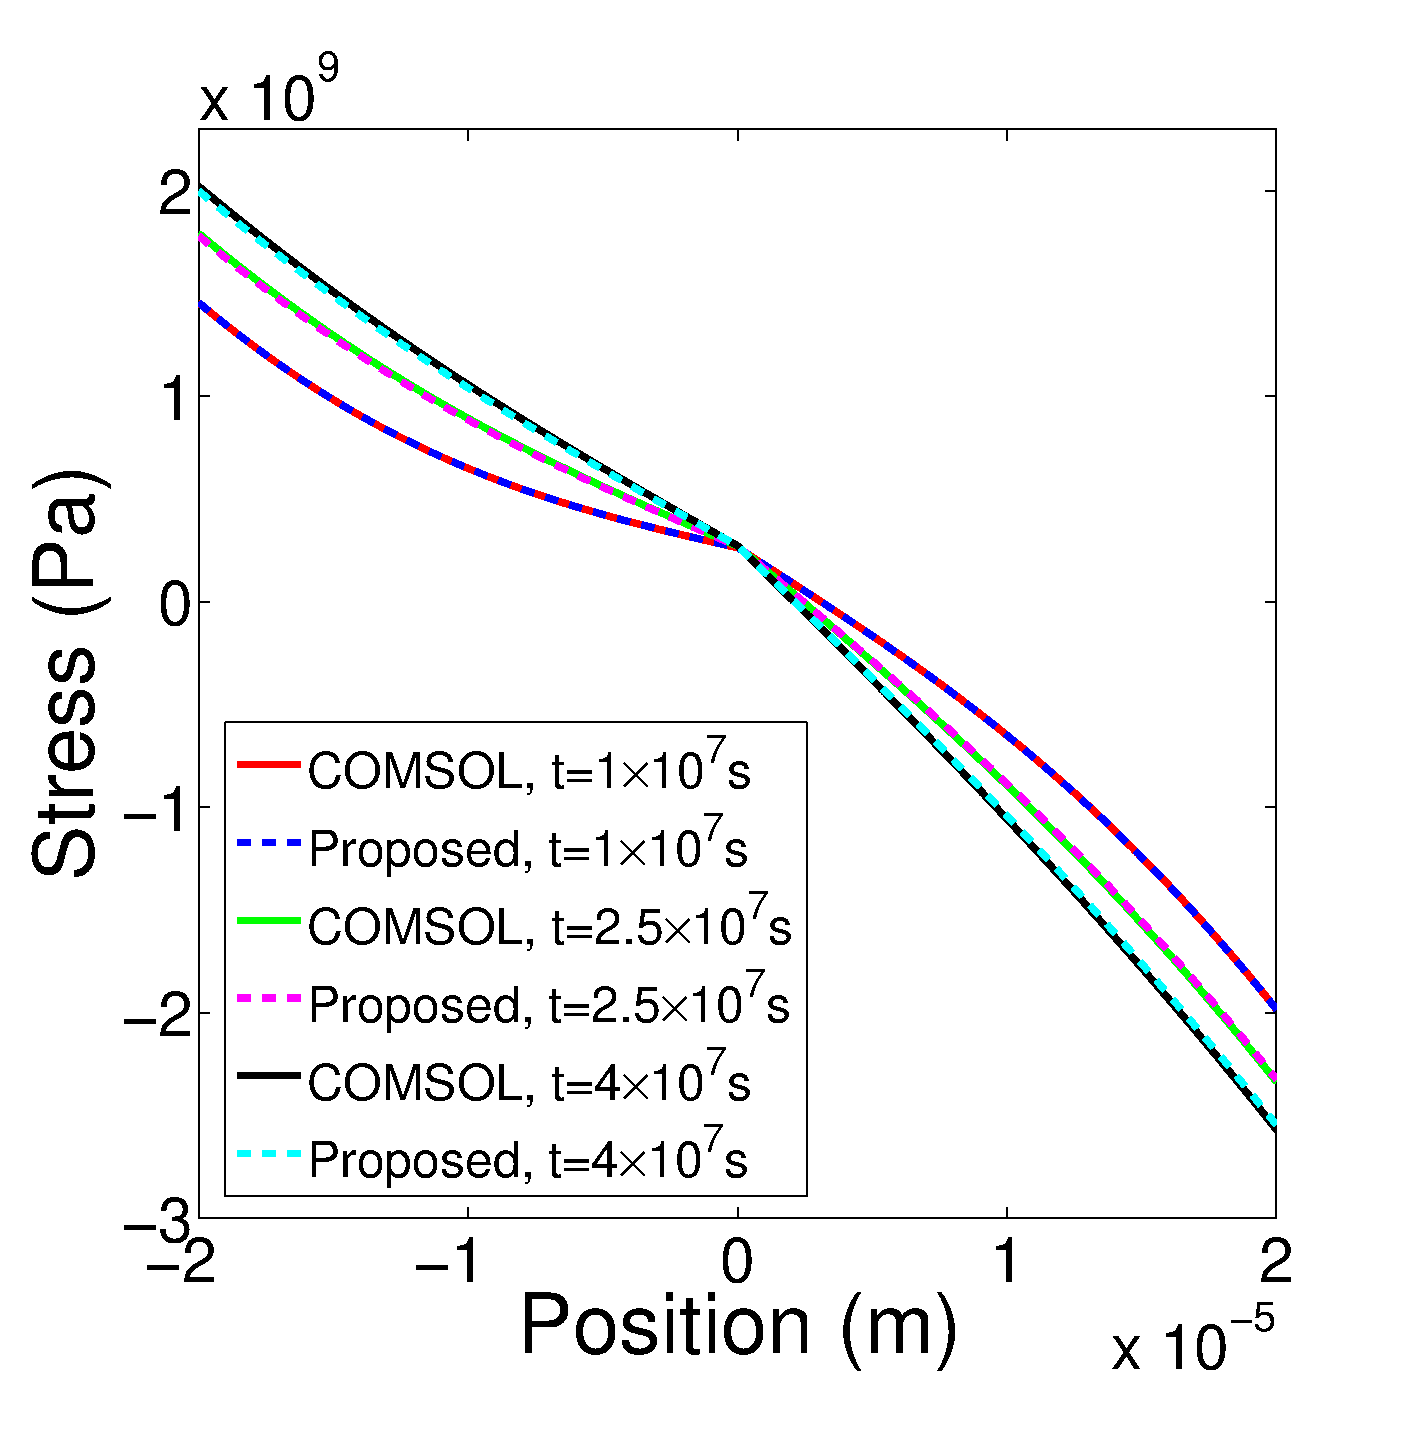
\includegraphics[width=0.45\columnwidth]{CStressMatComCompareT1.eps}
\label{fig:CT1Compare}}
\subfigure[]{
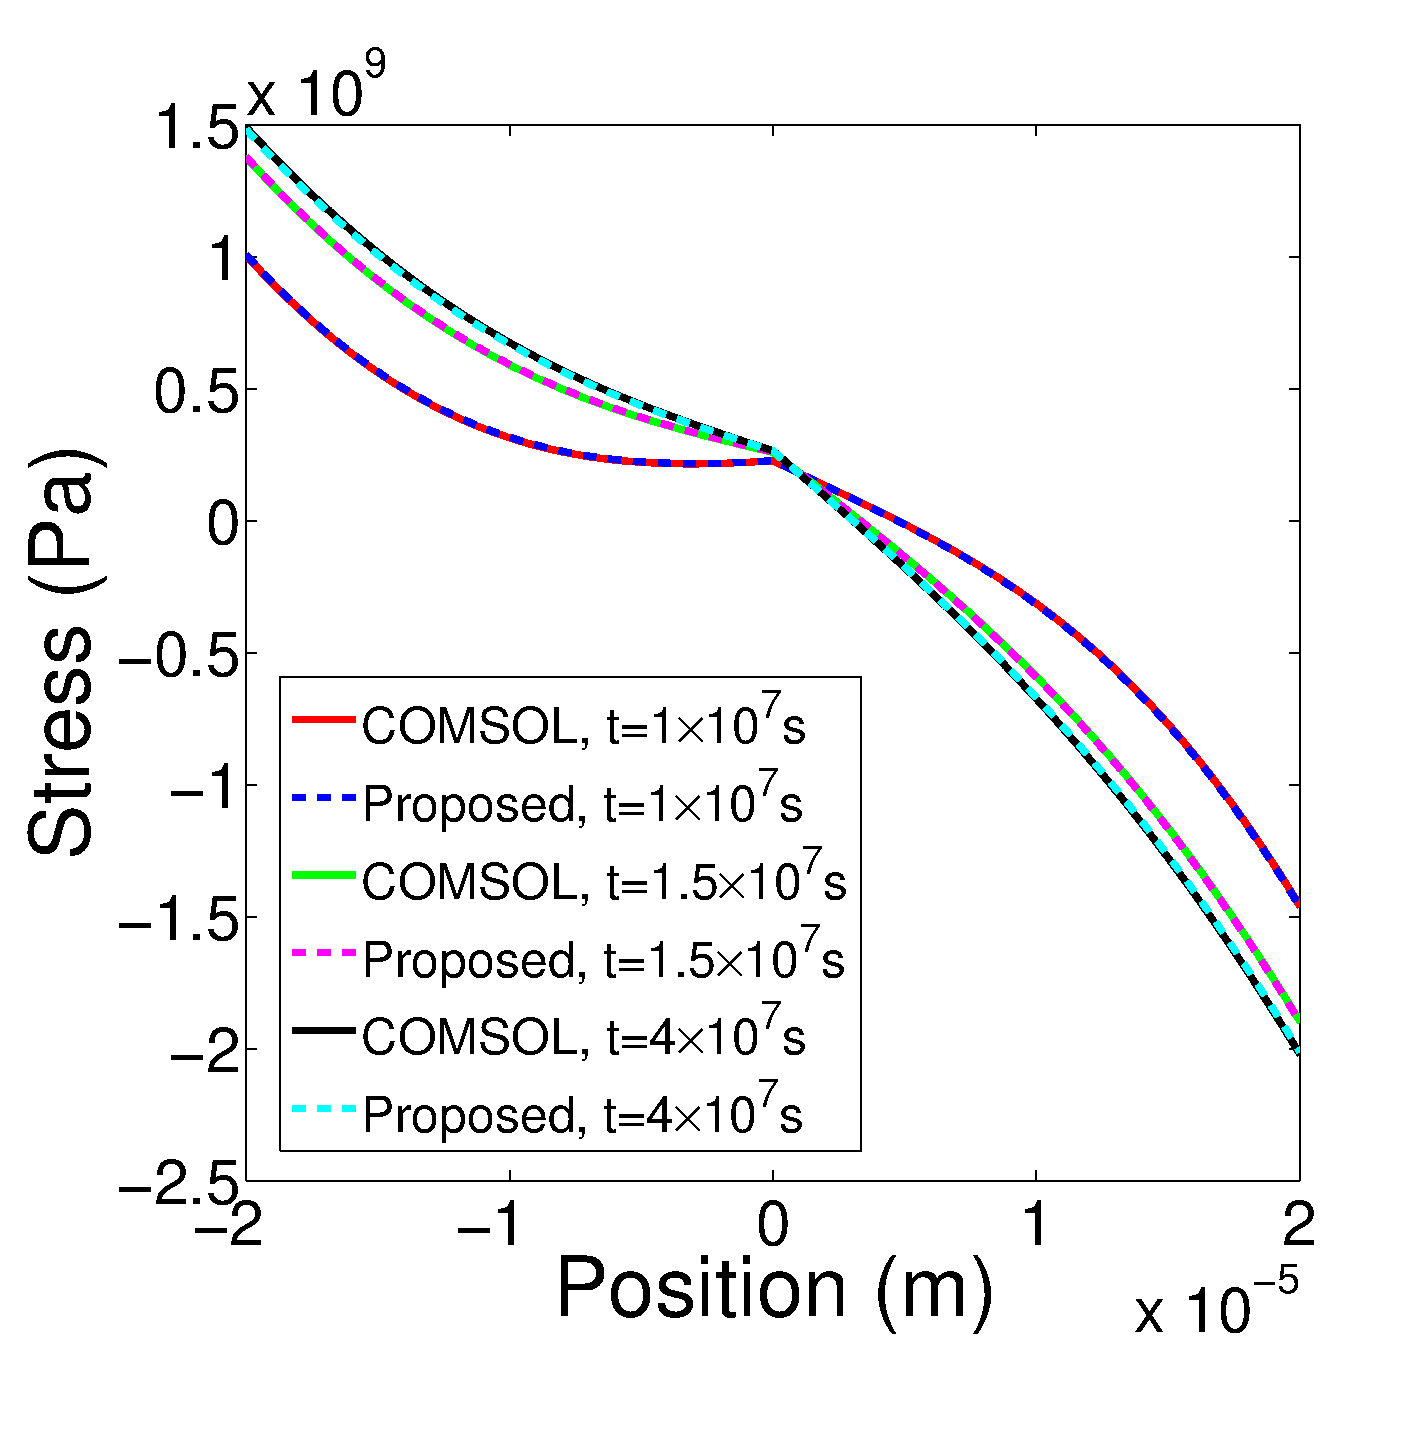
\includegraphics[width=0.45\columnwidth]{CStressMatComCompareT2.eps}
\label{fig:CT2Compare}}
\subfigure[]{
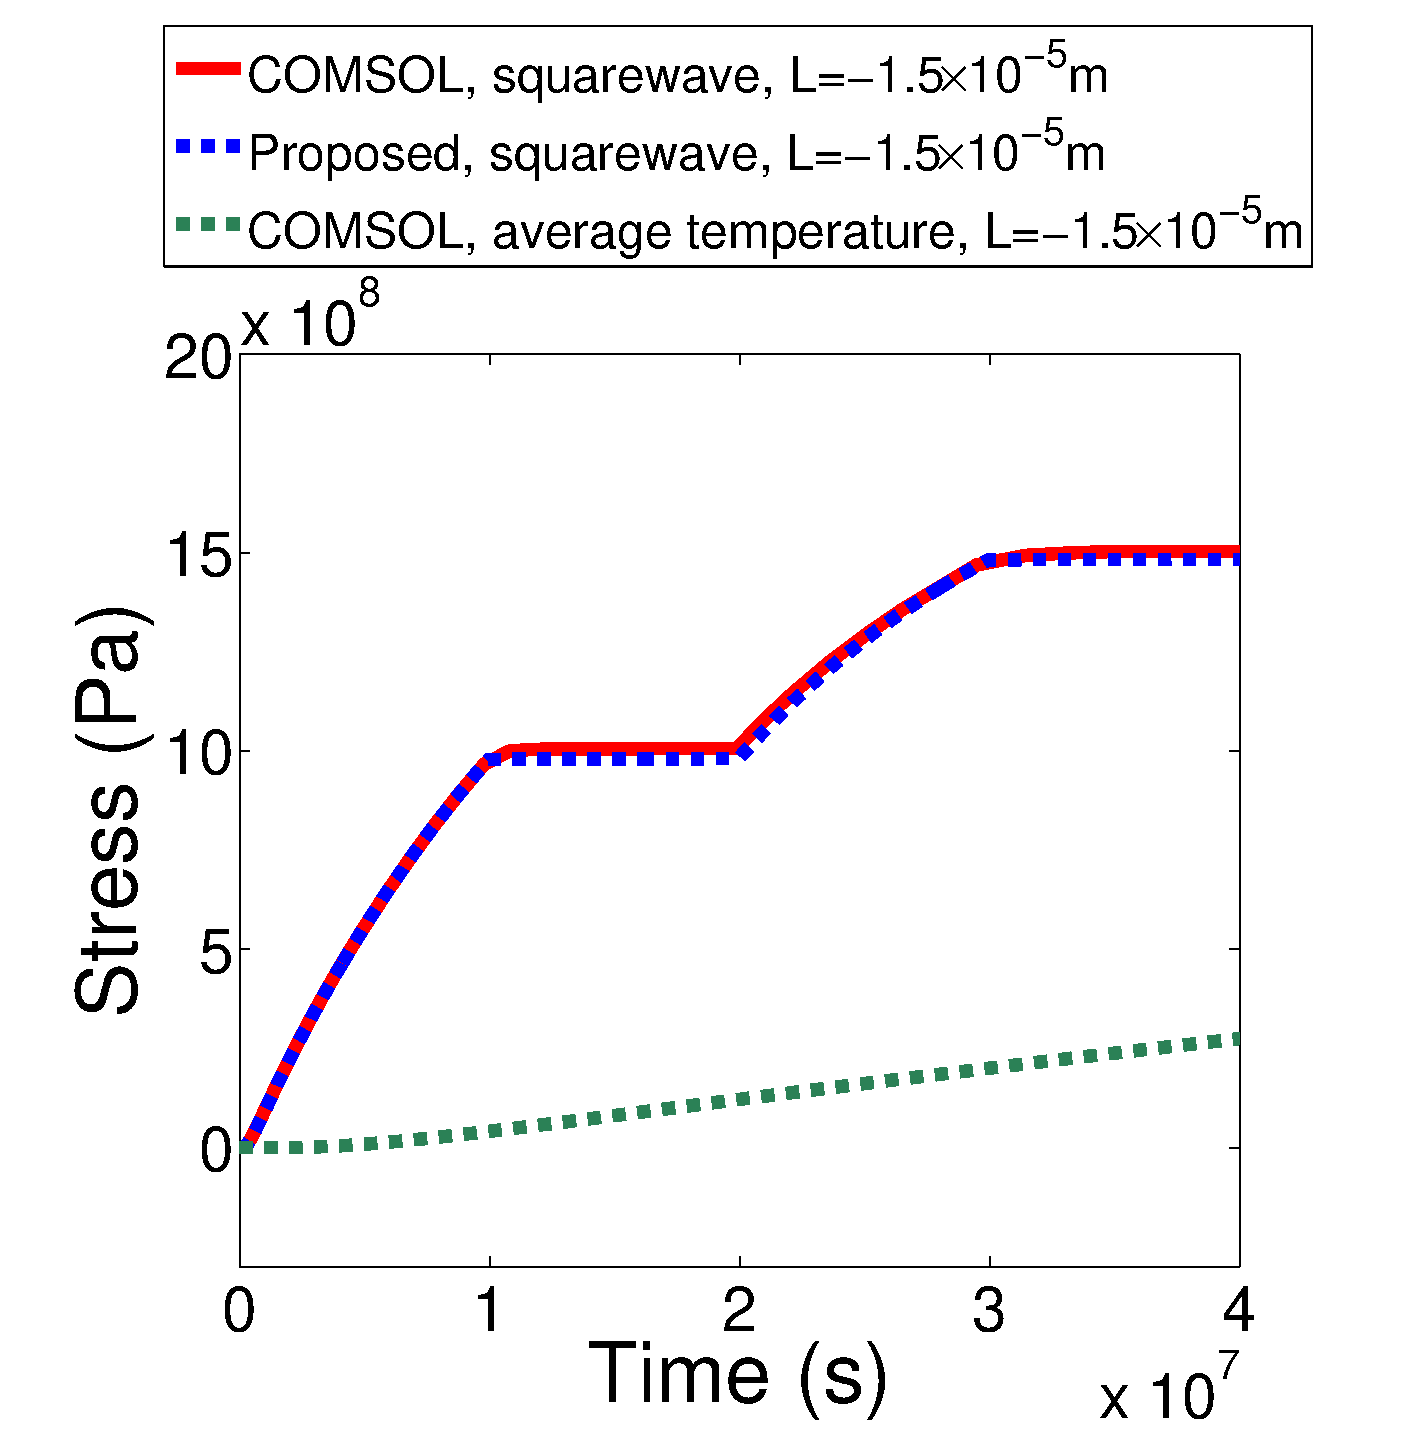
\includegraphics[width=0.45\columnwidth]{CLengthCompareT1.eps}
\label{fig:CT1Length}}
\subfigure[]{
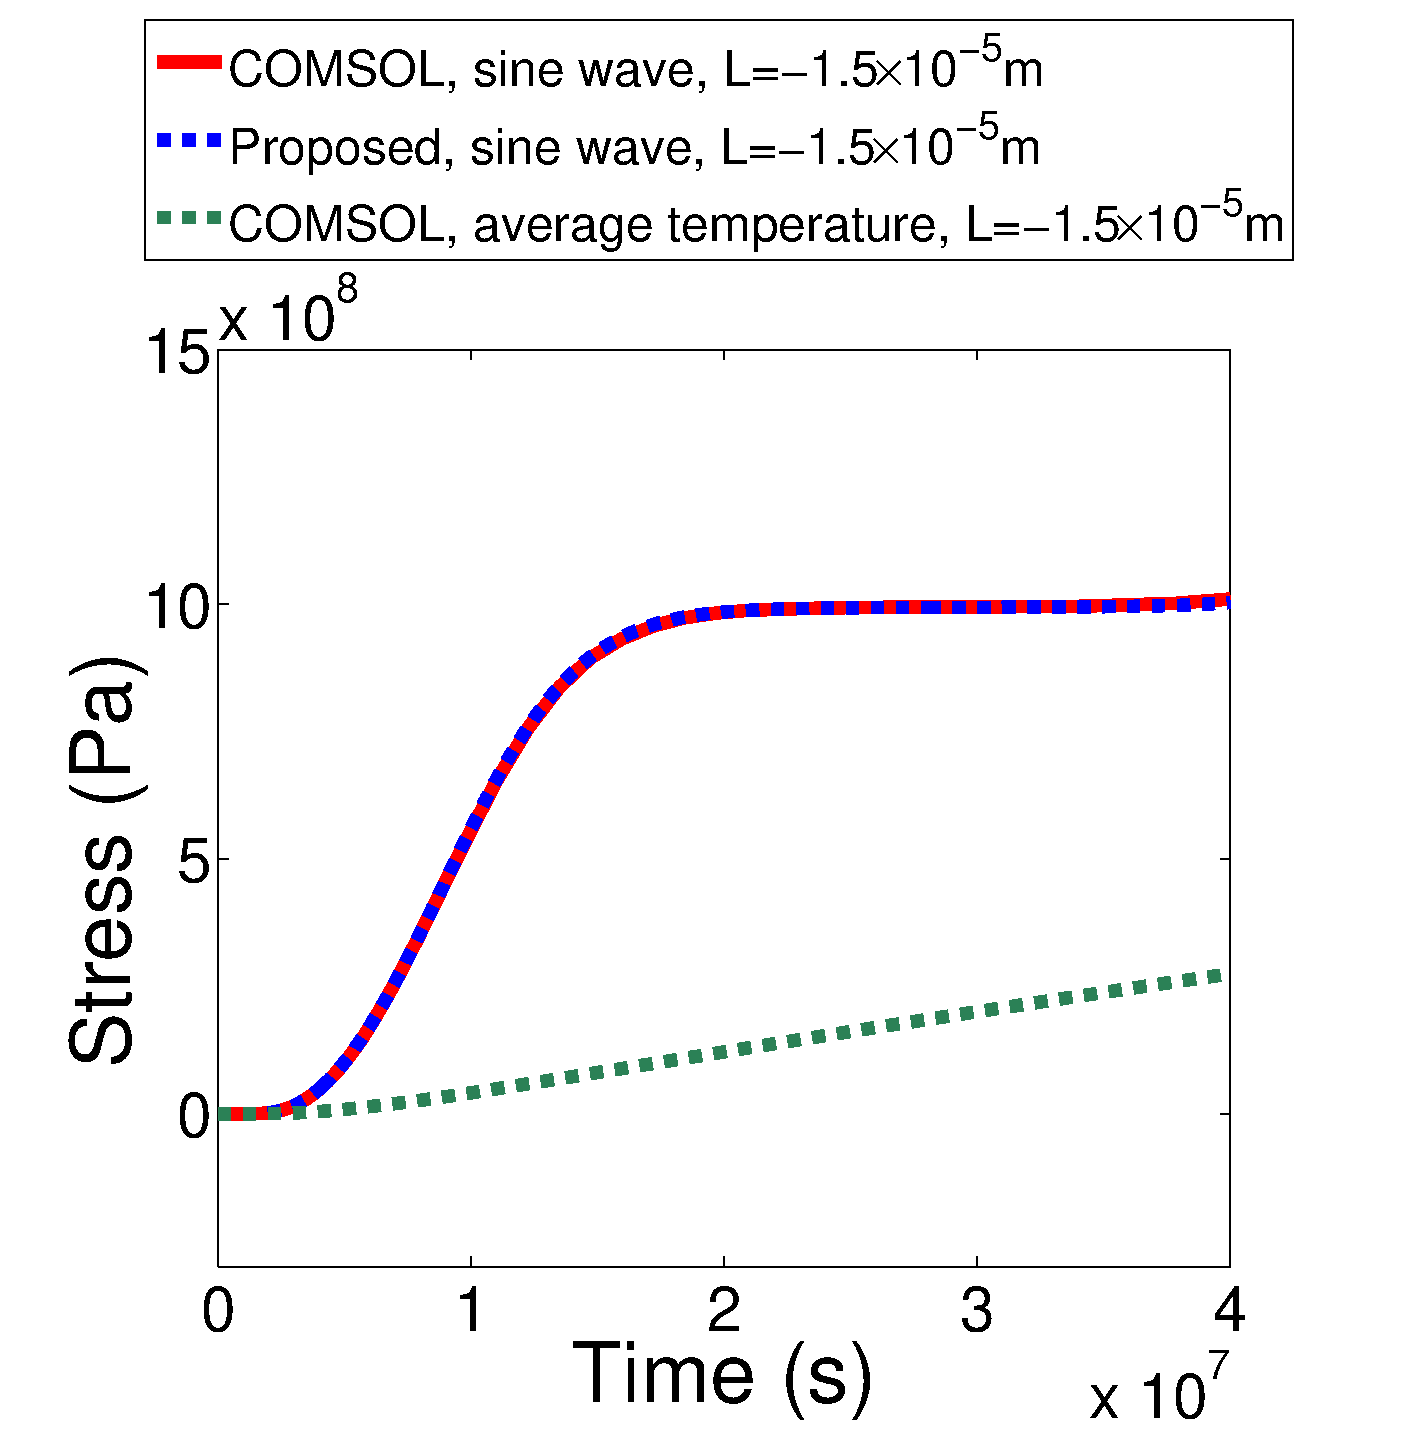
\includegraphics[width=0.45\columnwidth]{CLengthCompareT2.eps}
\label{fig:CT2Length}}
\caption{The experiments results of T-shaped interconnect tree at changing temperatures, $j_1=2\times10^{10}A/m^2,\;j_2=3\times10^{10}A/m^2,\;j_3=4\times10^{10}A/m^2,\;
j_4=5\times10^{10}A/m^2$ (a) the comparison of stress evolution at square wave temperature at a fixed time; (b) the comparison of stress evolution at sine wave temperature at a fixed time; (c) the comparison of stress evolution at square wave temperature at a fixed position; (d) the comparison of stress evolution at sine wave temperature at a fixed position}
\label{fig:CResults}
\end{figure}